\documentclass[12pt,english]{article}\usepackage[]{graphicx}\usepackage[]{xcolor}
% maxwidth is the original width if it is less than linewidth
% otherwise use linewidth (to make sure the graphics do not exceed the margin)
\makeatletter
\def\maxwidth{ %
  \ifdim\Gin@nat@width>\linewidth
    \linewidth
  \else
    \Gin@nat@width
  \fi
}
\makeatother

\definecolor{fgcolor}{rgb}{0.345, 0.345, 0.345}
\newcommand{\hlnum}[1]{\textcolor[rgb]{0.686,0.059,0.569}{#1}}%
\newcommand{\hlsng}[1]{\textcolor[rgb]{0.192,0.494,0.8}{#1}}%
\newcommand{\hlcom}[1]{\textcolor[rgb]{0.678,0.584,0.686}{\textit{#1}}}%
\newcommand{\hlopt}[1]{\textcolor[rgb]{0,0,0}{#1}}%
\newcommand{\hldef}[1]{\textcolor[rgb]{0.345,0.345,0.345}{#1}}%
\newcommand{\hlkwa}[1]{\textcolor[rgb]{0.161,0.373,0.58}{\textbf{#1}}}%
\newcommand{\hlkwb}[1]{\textcolor[rgb]{0.69,0.353,0.396}{#1}}%
\newcommand{\hlkwc}[1]{\textcolor[rgb]{0.333,0.667,0.333}{#1}}%
\newcommand{\hlkwd}[1]{\textcolor[rgb]{0.737,0.353,0.396}{\textbf{#1}}}%
\let\hlipl\hlkwb

\usepackage{framed}
\makeatletter
\newenvironment{kframe}{%
 \def\at@end@of@kframe{}%
 \ifinner\ifhmode%
  \def\at@end@of@kframe{\end{minipage}}%
  \begin{minipage}{\columnwidth}%
 \fi\fi%
 \def\FrameCommand##1{\hskip\@totalleftmargin \hskip-\fboxsep
 \colorbox{shadecolor}{##1}\hskip-\fboxsep
     % There is no \\@totalrightmargin, so:
     \hskip-\linewidth \hskip-\@totalleftmargin \hskip\columnwidth}%
 \MakeFramed {\advance\hsize-\width
   \@totalleftmargin\z@ \linewidth\hsize
   \@setminipage}}%
 {\par\unskip\endMakeFramed%
 \at@end@of@kframe}
\makeatother

\definecolor{shadecolor}{rgb}{.97, .97, .97}
\definecolor{messagecolor}{rgb}{0, 0, 0}
\definecolor{warningcolor}{rgb}{1, 0, 1}
\definecolor{errorcolor}{rgb}{1, 0, 0}
\newenvironment{knitrout}{}{} % an empty environment to be redefined in TeX

\usepackage{alltt}
\usepackage{mypreamble}
\usepackage{myRpreamble}
\IfFileExists{upquote.sty}{\usepackage{upquote}}{}
\begin{document}
{\bf Arkaraj Mukherjee}
{\bf Worksheet 7}
\\
\begin{knitrout}
\definecolor{shadecolor}{rgb}{0.969, 0.969, 0.969}\color{fgcolor}\begin{kframe}
\begin{alltt}
\hlkwd{library}\hldef{(}\hlsng{"tidyverse"}\hldef{);}
\hlkwd{library}\hldef{(}\hlsng{"data.table"}\hldef{);}
\end{alltt}
\end{kframe}
\end{knitrout}
\begin{enumerate}[label=\arabic*.]
\item
\begin{enumerate}[label=(\alph*)]
\item As $X_1,\ldots,X_n$ are all i.i.d, so are $f(X_1),\ldots,f(X_n)$ and these have mean,
$$\bE[X_i]=\int_{-\infty}^{\infty}x\cdot
P(f(X_i)=x)dx=\int_{-\infty}^{\infty}f(x)\cdot
P(X_i=x)dx$$
$$=\int_a^bf(x)P(X=x)dx=\int_a^bf(x)\cdot\frac{1}{b-a}dx=\frac{1}{b-a}\int_a^bf(x)dx$$
Using LOTUS and the fact that $X_i\sim\text{Unif}(a,b)$, now we can use the weak law of large numbers to say that for all $\epsilon/2>0$
$$P\qty(\left|\frac{1}{n}\sum_{i=1}^nf(X_i)-\frac{1}{b-a}\int_a^bf(x)dx\right|<\epsilon/2)\xrightarrow{n\to\infty}1$$
This implies that,
$$P\qty(\left|\frac{1}{n}\sum_{i=1}^nf(X_i)-\frac{1}{b-a}\int_a^bf(x)dx\right|
>\epsilon)=1-P\qty(\left|\overline{f(X)}-\frac{1}{b-a}\int_a^bf(x)dx\right|\leq\epsilon)$$
$$\leq
1-P\qty(\qty|\overline{f(X)}-\frac{1}{b-a}\int_a^bf(x)dx|\geq\epsilon/2)$$
$$=1-P\qty(\qty|\overline{f(X)}-\frac{1}{b-a}\int_a^bf(x)dx|<\epsilon/2)\xrightarrow{n\to\infty}1-1=0$$
\item
\begin{knitrout}
\definecolor{shadecolor}{rgb}{0.969, 0.969, 0.969}\color{fgcolor}\begin{kframe}
\begin{alltt}
\hldef{f} \hlkwb{=} \hlkwa{function}\hldef{(}\hlkwc{x}\hldef{) \{(}\hlnum{16}\hlopt{+}\hlkwd{sin}\hldef{(x))}\hlopt{/}\hldef{(x}\hlopt{^}\hlnum{2}\hlopt{+}\hlnum{4}\hldef{)\};}
\hldef{f} \hlkwb{=} \hlkwd{Vectorize}\hldef{(f);}
\hldef{Intapx} \hlkwb{=} \hlkwa{function}\hldef{(}\hlkwc{n}\hldef{) \{(}\hlnum{7}\hlopt{-}\hlnum{0}\hldef{)}\hlopt{*}\hlkwd{mean}\hldef{(}\hlkwd{f}\hldef{(}\hlkwd{runif}\hldef{(n,}\hlkwc{min}\hldef{=}\hlnum{0}\hldef{,}\hlkwc{max}\hldef{=}\hlnum{7}\hldef{)))\};}
\hldef{I_hat} \hlkwb{=} \hlkwd{mean}\hldef{(}\hlkwd{replicate}\hldef{(}\hlnum{100}\hldef{,\{}\hlkwd{Intapx}\hldef{(}\hlnum{50}\hldef{)\}))}
\hldef{I_hat}
\end{alltt}
\begin{verbatim}
## [1] 10.58111
\end{verbatim}
\end{kframe}
\end{knitrout}
\item
\begin{knitrout}
\definecolor{shadecolor}{rgb}{0.969, 0.969, 0.969}\color{fgcolor}\begin{kframe}
\begin{alltt}
\hlkwd{integrate}\hldef{(f,}\hlnum{0}\hldef{,}\hlnum{7}\hldef{)}\hlopt{$}\hldef{value}
\end{alltt}
\begin{verbatim}
## [1] 10.58204
\end{verbatim}
\begin{alltt}
\hlkwd{abs}\hldef{(I_hat} \hlopt{-} \hlkwd{integrate}\hldef{(f,}\hlnum{0}\hldef{,}\hlnum{7}\hldef{)}\hlopt{$}\hldef{value)}
\end{alltt}
\begin{verbatim}
## [1] 0.0009285878
\end{verbatim}
\end{kframe}
\end{knitrout}
\end{enumerate}
\begin{enumerate}[label=(\alph*)]
\item As $X$ is the number of marked fish in a sample of size $20$ from  a population of $N$ fish where $50$ are marked and thus $N-50$ unmarked, it must follow $\text{Hypergeom}(50,N-50,20)$.
\item 
\begin{knitrout}
\definecolor{shadecolor}{rgb}{0.969, 0.969, 0.969}\color{fgcolor}\begin{kframe}
\begin{alltt}
\hldef{N} \hlkwb{=} \hlnum{50}\hldef{;}
\hldef{X} \hlkwb{=} \hlkwd{rhyper}\hldef{(}\hlnum{100}\hldef{,}\hlnum{50}\hldef{,N}\hlopt{-}\hlnum{50}\hldef{,}\hlnum{20}\hldef{);}
\hlkwd{head}\hldef{(X,}\hlkwc{n}\hldef{=}\hlnum{10}\hldef{)}
\end{alltt}
\begin{verbatim}
##  [1] 20 20 20 20 20 20 20 20 20 20
\end{verbatim}
\end{kframe}
\end{knitrout}
\item The biologist would write  $X/20=50/\hat{N}$ and thus $\hat{N}=1000/X$
\item
\begin{knitrout}
\definecolor{shadecolor}{rgb}{0.969, 0.969, 0.969}\color{fgcolor}\begin{kframe}
\begin{alltt}
\hldef{Sim} \hlkwb{=} \hlkwa{function}\hldef{(}\hlkwc{N}\hldef{) \{}\hlkwd{rhyper}\hldef{(}\hlnum{1000}\hldef{,}\hlnum{50}\hldef{,N}\hlopt{-}\hlnum{50}\hldef{,}\hlnum{20}\hldef{)\}}
\hldef{dat} \hlkwb{=} \hlkwd{data.table}\hldef{(} \hlkwc{id} \hldef{=} \hlnum{1}\hlopt{:}\hlnum{7}\hldef{,} \hlkwc{N} \hldef{=} \hlkwd{c}\hldef{(}\hlnum{50}\hldef{,}\hlkwd{seq}\hldef{(}\hlnum{100}\hldef{,}\hlnum{500}\hldef{,}\hlkwc{by}\hldef{=}\hlnum{100}\hldef{),}\hlnum{1000}\hldef{))}
\hldef{dat}\hlopt{$}\hldef{X} \hlkwb{=} \hlkwd{lapply}\hldef{(dat}\hlopt{$}\hldef{N,Sim)}
\hldef{dat}\hlopt{$}\hldef{N} \hlkwb{=} \hlkwd{lapply}\hldef{(dat}\hlopt{$}\hldef{X,}\hlkwa{function}\hldef{(}\hlkwc{x}\hldef{)\{}\hlnum{1000}\hlopt{/}\hldef{x[x}\hlopt{>}\hlnum{0}\hldef{]\})}
\hldef{dat}\hlopt{$}\hldef{E} \hlkwb{=} \hlkwd{sapply}\hldef{(dat}\hlopt{$}\hldef{N,mean)}
\hldef{dat}\hlopt{$}\hldef{Var} \hlkwb{=} \hlkwd{sapply}\hldef{(dat}\hlopt{$}\hldef{N,var)}
\hlkwd{ggplot}\hldef{(dat,} \hlkwd{aes}\hldef{(}\hlkwc{x} \hldef{= id))} \hlopt{+}
\hlkwd{geom_point}\hldef{(}\hlkwd{aes}\hldef{(}\hlkwc{y} \hldef{= dat}\hlopt{$}\hldef{E))}
\end{alltt}
\end{kframe}
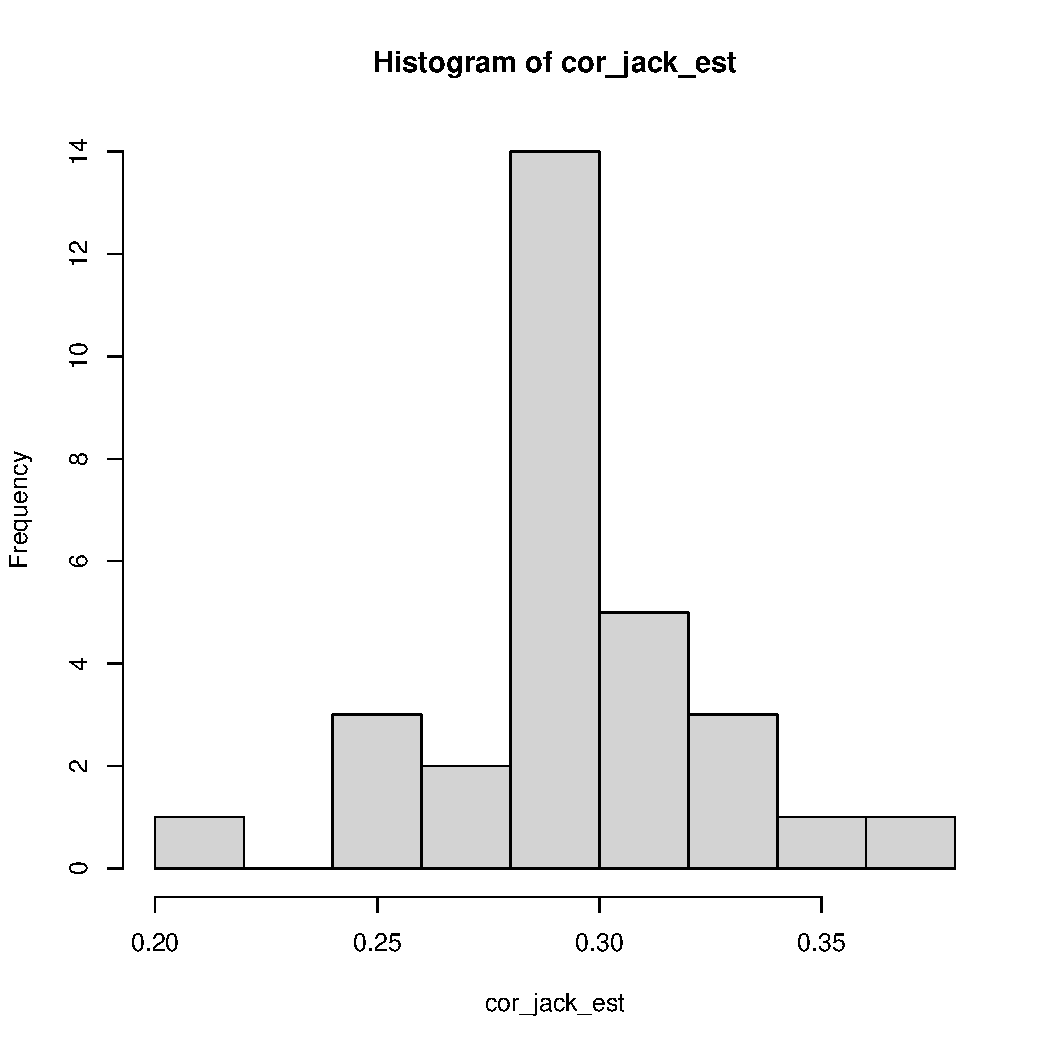
\includegraphics[width=\maxwidth]{figure/unnamed-chunk-5-1} 
\begin{kframe}\begin{alltt}
\hlkwd{ggplot}\hldef{(dat,} \hlkwd{aes}\hldef{(}\hlkwc{x} \hldef{= id))} \hlopt{+}
\hlkwd{geom_point}\hldef{(}\hlkwd{aes}\hldef{(}\hlkwc{y} \hldef{= Var))}
\end{alltt}
\end{kframe}
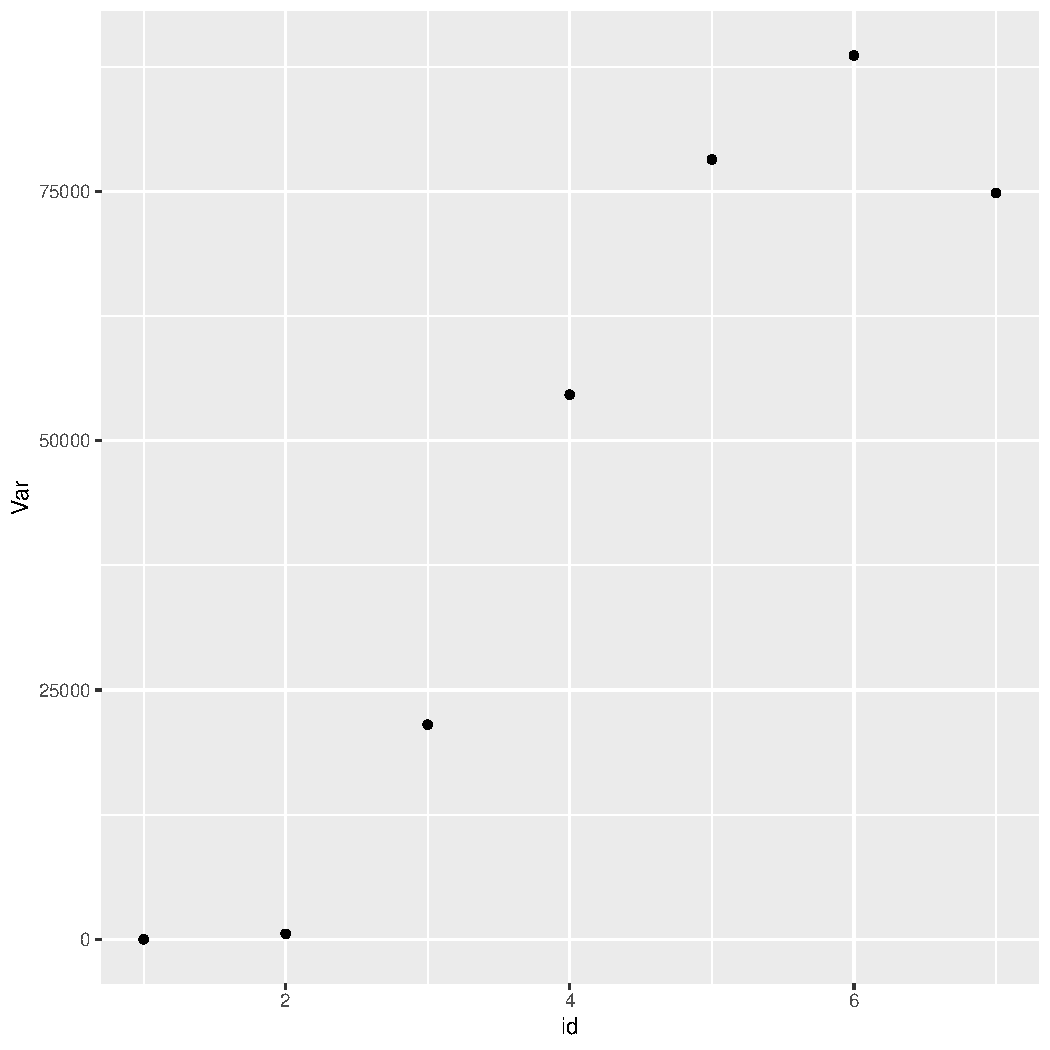
\includegraphics[width=\maxwidth]{figure/unnamed-chunk-5-2} 
\end{knitrout}
\end{enumerate}
\end{enumerate}
\end{document}
